%%%%%%%%%%%%%%%%%%%%%%%%%%%%%%%%%%%%%%%%%%%%%%%%%%%%%%%%%%
%% BEGIN PREAMBLE
\documentclass[10pt]{article}

%%%% Sets 1 inch margins on document
\usepackage[margin=1in]{geometry}

%%%% For math macros
\usepackage{amsmath}

%%%% Needed for including figures and other images
\usepackage{graphicx}

%%%% Adds ability to adjust document vertical spacing
% usage:
%   \setspace{1.5} % 1.5x for line spacing
\usepackage{setspace}

%%%% Needed for specifying the list items in enumerate env
% eg. (a,b,b) or (i,ii,iii), (1,2,3)
% usage:
%   \begin{enumerate} [label=(\alph*)] % for (a), (b), (c)
\usepackage{enumitem}

%%%% Defines Times New Roman as font
  % for math and text environments
\usepackage{newtxtext,newtxmath}

%%%% For H float option when inserting figure
%   [H] inserts figure _exactly_ where it is typeset
% usage:
%   begin{figure} [H]
\usepackage{float}

%%%% For fancy header and footer ;)
\usepackage{fancyhdr}
\pagestyle{fancy}
\fancyhead[LO,L]{Samuel Barton}
\fancyhead[CO,C]{ENGS31 - Lab 4}
\fancyhead[RO,R]{\today}
\fancyfoot[LO,L]{}
\fancyfoot[CO,C]{\thepage}
\fancyfoot[RO,R]{}
\renewcommand{\headrulewidth}{0.4pt}
\renewcommand{\footrulewidth}{0.4pt}

%%%% Setting margins in tabular environments
% For making equations (esp. fractions) fit in cells vertically
\usepackage{cellspace}
\cellspacetoplimit 4pt
\cellspacebottomlimit 4pt

%%%% Minted for vhdl snippets
\usepackage[cachedir=cache]{minted}
\setminted{fontsize=\small,baselinestretch=0.65,linenos}
%% END PREAMBLE %%
%%%%%%%%%%%%%%%%%%%%%%%%%%%%%%%%%%%%%%%%%%%%%%%%%%%%%%%%%%%%%%%

\begin{document}

\setstretch{1.25} % set spacing to 1.25x

% Assignment Name
\begin{centering}
  \section*{LAB 4}
\end{centering}

\subsection*{Deliverable 2: Generate an 8Hz Clock}

We need a value $ CLOCK\_DIVIDER\_TC := 6.25 \times 10^6 $, which requires 23 bits.

\subsection*{Deliverable 3: Testbench and Screenshots}

\subsubsection*{Testing Plan}

\begin{enumerate}
  \item Wait off for a few clock cycles. All LEDs should be off.
  \item Flip both switches to test hazard mode. All LEDs should blink on and off simultaneously.
  \item Test right turn by setting the left\_switch low. We should see the cascading R* LEDs.
  \item Test the left turn by flipping the right switch off and switching the left switch on. Also test that the signal runs to completion by flipping right switch on mid turn signal. 
\end{enumerate}

\subsubsection*{Annotated Screenshot of Simulation}

\begin{figure} [H]
  \center
  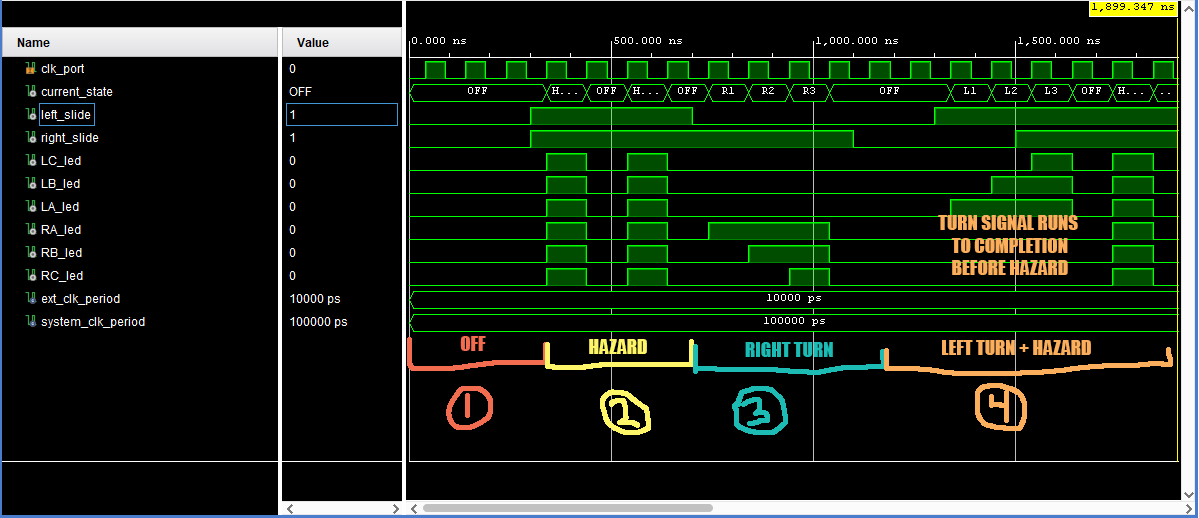
\includegraphics[width=0.9\textwidth]{figures/simulation_annotated.png}
  \caption{Annotated Simulation Screenshot}
\end{figure}

\subsubsection*{VHDL Testbench}

On Canvas.

\subsection*{Deliverable 4: Constrain File}

On canvas.

\subsection*{Deliverable 5: Program the FPGA}

\begin{figure} [H]
  \center
  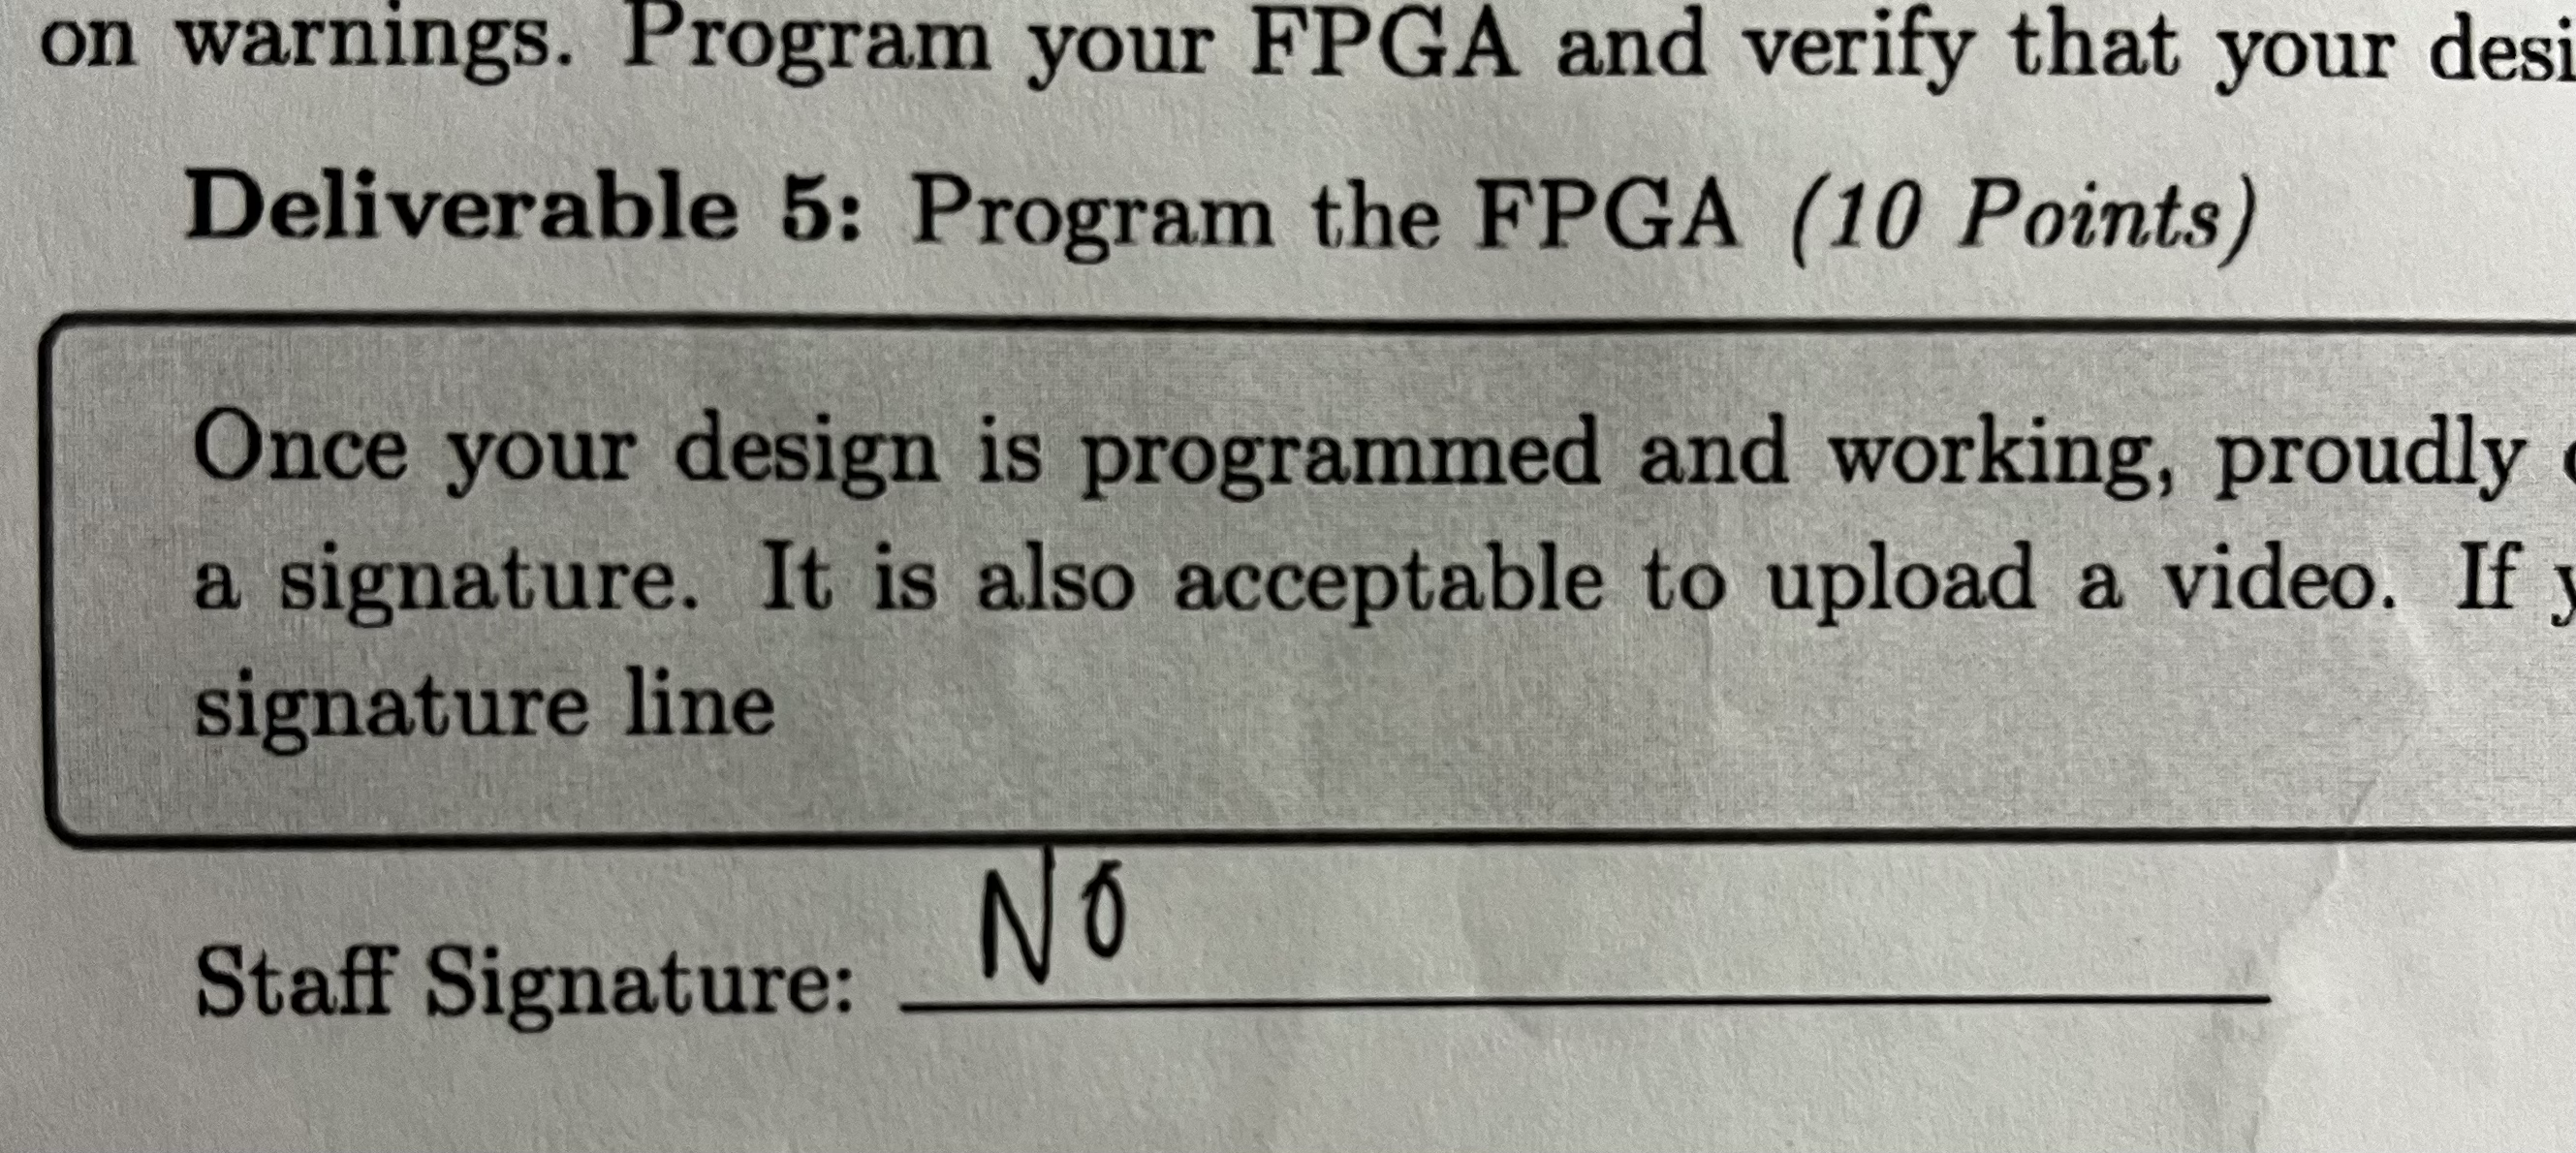
\includegraphics[width=0.5\textwidth]{figures/signature.png}
  \caption{TA Signature}
\end{figure}

\subsection*{Deliverable 6: Final Design}

\begin{figure} [H]
  \center
  \includegraphics[width=0.95\textwidth]{figures/fsm.png}
  \caption{Final State Machine Diagram}
\end{figure}

\end{document}

